\documentclass[conference]{IEEEtran}

\usepackage{cite}
\usepackage{amsmath,amssymb,amsfonts}
\usepackage{graphicx}
\usepackage{booktabs}
\usepackage{url}
\usepackage{xcolor}
\usepackage{tikz}
\usetikzlibrary{arrows.meta,positioning,shapes.geometric,calc,fit,backgrounds}
\usepackage{pgfplots}
\pgfplotsset{compat=1.17}

\begin{document}

\title{Evaluating Hybrid Retrieval Strategies in\\
Enterprise Retrieval-Augmented Generation Systems:\\
A Comparative Study}

\author{%
\IEEEauthorblockN{Yasharth Singh}
\IEEEauthorblockA{%
Dept. of Computer Science and Engineering\\
Jaypee Institute of Information Technology\\
Noida, India\\
\texttt{yasharthsingh0910@gmail.com}}

}

\maketitle

\begin{abstract}
Enterprise knowledge platforms increasingly rely on retrieval-augmented
generation (RAG) to answer employee questions over internal documents, where
retrieval quality, not generation, is the dominant bottleneck for factual
grounding. We present Pragya, an enterprise RAG system built on FastAPI,
PostgreSQL, and the Qdrant vector database, and use it as a controlled testbed
to compare three retrieval strategies on a real corporate corpus: (A) dense
semantic retrieval, (B) hybrid dense$+$sparse retrieval fused with reciprocal
rank fusion (RRF), and (C) hybrid retrieval followed by cross-encoder
reranking. Pragya uses hierarchical chunking, asymmetric Gemini embeddings
truncated to 768 dimensions, and a three-tier access-control filter enforced at
the vector-database layer. We evaluate all three strategies on a fixed
seven-document corpus and 30 ground-truth question--answer pairs, scoring
faithfulness and context precision with two \emph{independent} judge models
distinct from the answer generator, eliminating self-evaluation bias. Hybrid
retrieval attains the best average score (0.914), ahead of dense (0.903) on
\emph{both} metrics, though by small margins (faithfulness 0.890 vs.\ 0.873;
context precision 0.939 vs.\ 0.933); the sparse channel is active, changing the
retrieved context on all 30 questions. Reranking is clearly worst (0.840): its
faithfulness drops from 0.873 (dense) to 0.777. We trace this to over-pruning:
on a small, clean corpus the cross-encoder, combined with a per-source diversity
cap and parent-chunk deduplication, reduces the generator's context to about
four blocks. Our results push back on the assumption that reranking is uniformly
beneficial and show that the value of each retrieval stage is contingent on
corpus characteristics.
\end{abstract}

\begin{IEEEkeywords}
retrieval-augmented generation, hybrid retrieval, reciprocal rank fusion,
reranking, enterprise search, RAGAS.
\end{IEEEkeywords}

\section{Introduction}
Modern organizations accumulate large volumes of internal documents, such as
human resources policies, security standards, finance procedures, and
engineering handbooks. Their answers are nominally available to employees but
practically inaccessible: finding "how many casual leaves do I get?" means knowing which
document to open and where to look. Retrieval-augmented generation (RAG)
\cite{lewis2020retrieval} offers a natural interface to this knowledge: an employee asks
in natural language, relevant passages are retrieved from a corpus, and a large
language model (LLM) composes a grounded answer with citations.

In such systems the generation model is rarely the limiting factor. Given
correct supporting passages, a modern LLM produces fluent, faithful answers; the
risk of hallucination is driven instead by \emph{whether the right passages were
retrieved at all}. Retrieval quality is therefore the bottleneck for trustworthy
enterprise answering, and the choice of retrieval strategy is the central design
decision.

Three strategies dominate current practice. \emph{Dense} retrieval embeds the
query and documents into a shared vector space and ranks by semantic similarity.
\emph{Hybrid} retrieval additionally runs a sparse, keyword-oriented retriever
(such as BM25 \cite{robertson2009probabilistic}) and fuses the two ranked lists, typically with
reciprocal rank fusion (RRF) \cite{cormack2009reciprocal}, on the intuition that semantic and
lexical matching are complementary. \emph{Reranking} adds a cross-encoder
\cite{nogueira2019passage} that jointly scores each (query, passage) pair and reorders
the fused candidates, trading compute for precision. The prevailing assumption is
that each added stage monotonically improves answer quality.

We test that assumption empirically. Using Pragya, a working enterprise RAG
platform whose retrieval core implements all three strategies behind a single
interface, we run a controlled comparison on a real enterprise corpus of seven
documents and 30 ground-truth question--answer pairs. We
evaluate faithfulness and context precision with two judge models that are
\emph{independent} of the answer generator, which removes the self-evaluation
bias that arises when a model grades its own output.

Our contributions are:
\begin{itemize}
  \item A controlled, three-way comparison (dense vs. hybrid vs.
        hybrid$+$rerank) on a real enterprise corpus, holding chunking,
        embeddings, generator, and access control fixed across conditions.
  \item A bias-free evaluation design using two independent judge models, with
        a transparent account of its asymmetries.
  \item An empirical finding that contradicts the "reranking always helps"
        default: on a small, clean corpus, cross-encoder reranking degrades
        faithfulness by 0.10 absolute through context over-pruning, while hybrid
        retrieval yields a small but consistent gain over dense on both metrics,
        so retrieval-stage value is corpus-dependent.
\end{itemize}


\section{Related Work}
\textbf{Retrieval-augmented generation.} RAG couples a parametric generator with
a non-parametric retriever so that answers can be grounded in an external corpus
and updated without retraining \cite{lewis2020retrieval}.
This grounding is what makes citations and faithfulness measurable, and it
motivates the citation-enforced prompting we adopt (Section~\ref{sec:methods}).

\textbf{Dense retrieval.} Dual-encoder dense retrievers embed queries and
passages independently and rank by inner product or cosine similarity, capturing
semantic similarity beyond surface lexical overlap \cite{karpukhin2020dense}.
Pragya uses an asymmetric embedding scheme in which queries and documents declare
distinct task roles to share a common space.

\textbf{Sparse and lexical retrieval.} BM25 \cite{robertson2009probabilistic} remains a strong
keyword-matching baseline, particularly for exact tokens such as abbreviations
and identifiers that have weak semantic neighbourhoods.
Learned sparse encoders such as SPLADE extend this idea with neural term
weighting \cite{formal2021splade};
our implementation uses a lightweight hashed term-frequency approximation rather
than a learned encoder (Section~\ref{sec:methods}).

\textbf{Rank fusion.} Reciprocal rank fusion combines multiple ranked lists using
only rank position, requiring no score normalization or tuned weights
\cite{cormack2009reciprocal}.
We adopt RRF with the standard constant $k=60$.

\textbf{Cross-encoder reranking.} Cross-encoders jointly encode the (query,
passage) pair, allowing token-level attention across both and yielding higher
ranking precision at greater cost; they are typically applied to a shortlist
produced by a cheaper first-stage retriever \cite{nogueira2019passage}.
We use the \texttt{ms-marco-MiniLM-L-6-v2} cross-encoder.

\textbf{RAG evaluation.} RAGAS \cite{es2024ragas} provides reference-light metrics
for RAG systems, including faithfulness and context precision, computed by an
LLM judge.
We follow the spirit of these metrics but deliberately use judge models distinct
from the generator to avoid self-evaluation bias, a concern raised in the
LLM-as-a-judge literature \cite{zheng2023judging}.

\section{System Architecture}
Pragya is a three-layer asynchronous backend (FastAPI, Python~3.11) with a strict
separation between HTTP routing, business-logic services, and the data layer.
Document metadata and chat history are stored in a serverless PostgreSQL database
(Neon); document vectors are stored in Qdrant. Answer generation uses Gemini
Flash. The remainder of this section describes the components that bear on
retrieval quality; Fig.~\ref{fig:system} shows the end-to-end pipeline.

\subsection{Ingestion and hierarchical chunking}
Uploaded documents (PDF, DOCX, PPTX) are parsed page-by-page with PyMuPDF,
\texttt{python-docx}, and \texttt{python-pptx} respectively, preserving page
numbers so that citations can name an exact source page. Parsed text is then
de-boilerplated: lines that recur on more than 60\% of pages (letterhead,
classification banners, footers) and short structural labels are removed, because
repeated boilerplate makes chunks from different documents look spuriously
similar and dilutes both embeddings and reranking.

Cleaned text is split using \emph{hierarchical chunking}. We approximate token
counts with word counts (1 token $\approx$ 0.75 words). Each document is divided
into non-overlapping \emph{parent} chunks of 1365 words ($\approx$1024 tokens),
and each parent is sub-divided into overlapping \emph{child} chunks of 341 words
($\approx$256 tokens) with a 68-word ($\approx$20\%) overlap. Only child chunks
are embedded and retrieved (for precision); the corresponding parent chunk is
what the generator ultimately reads (for context). A document shorter than one
child chunk is stored whole as both its own child and parent, avoiding empty
parents.

\subsection{Embeddings}
Child chunks are embedded with \texttt{gemini-embedding-001}. The model's native
3072-dimensional output is truncated to 768 dimensions via Matryoshka
representation, reducing index size and search cost while preserving quality;
cosine distance makes re-normalization unnecessary. Embedding is
\emph{asymmetric}: documents are embedded with the task role
\texttt{retrieval\_document} at ingestion, while queries are embedded with
\texttt{retrieval\_query} at search time, so the two populate a shared space
correctly.

\subsection{Vector store and access control}
All vectors live in a single Qdrant collection (\texttt{pragya\_docs}) configured
with two \emph{named} vectors per point: a dense vector (768-d, cosine) and a
sparse vector for keyword matching. Each point also carries a payload with
\texttt{document\_id}, \texttt{department\_id}, \texttt{visibility},
\texttt{uploaded\_by}, \texttt{chunk\_index}, \texttt{parent\_text},
\texttt{source\_filename}, and \texttt{page\_number}.

Access control is enforced at the vector-database layer, not in application code.
Every retrieval query is wrapped in a three-tier visibility filter expressed as a
disjunction of three conjunctive sub-filters: \emph{company}-visible chunks
(any department), \emph{department}-visible chunks matching the caller's
department, and \emph{personal} chunks owned by the caller. A user can therefore
never retrieve a passage they are not authorized to see, regardless of the
retrieval strategy in use.

\begin{figure*}[t]
\centering
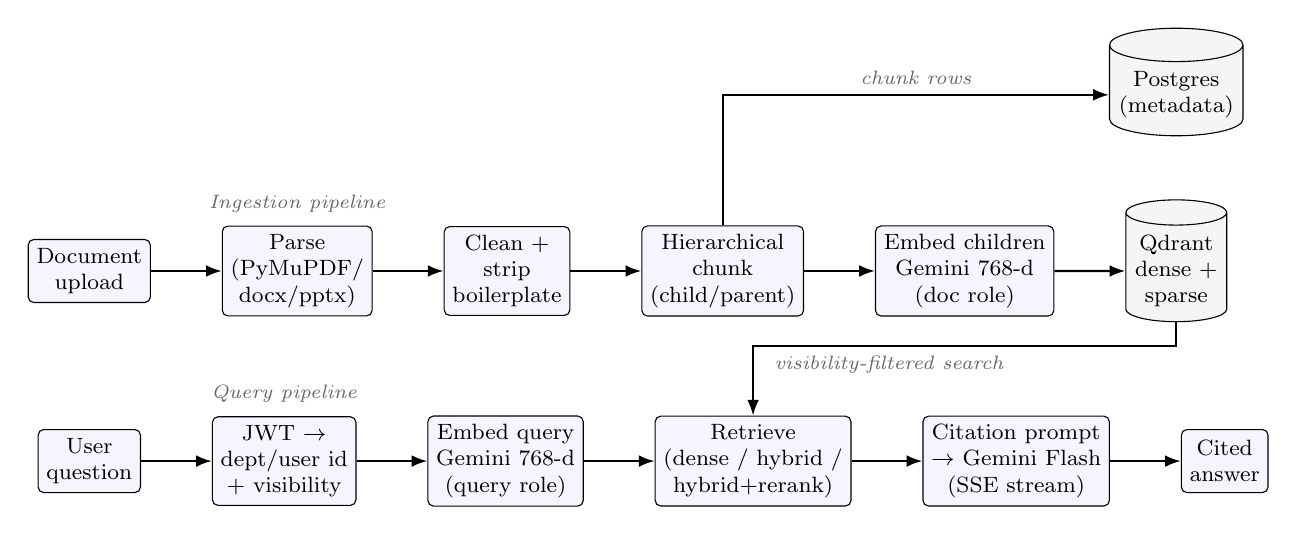
\begin{tikzpicture}[
  node distance=6mm and 9mm,
  box/.style={draw, rounded corners=2pt, align=center, font=\footnotesize,
              minimum height=8mm, inner sep=3pt, fill=blue!4},
  store/.style={draw, cylinder, shape border rotate=90, aspect=0.25,
                align=center, font=\footnotesize, fill=gray!8, minimum height=10mm},
  arr/.style={-{Latex[length=2mm]}, thick},
  lbl/.style={font=\scriptsize\itshape, text=black!60}
]
\node[box] (upload) {Document\\upload};
\node[box, right=of upload] (parse) {Parse\\(PyMuPDF/\\docx/pptx)};
\node[box, right=of parse] (clean) {Clean +\\strip\\boilerplate};
\node[box, right=of clean] (chunk) {Hierarchical\\chunk\\(child/parent)};
\node[box, right=of chunk] (embedd) {Embed children\\Gemini 768-d\\(doc role)};
\node[store, right=of embedd] (qdrant) {Qdrant\\dense +\\sparse};
\node[store, above=8mm of qdrant] (pg) {Postgres\\(metadata)};

\draw[arr] (upload) -- (parse);
\draw[arr] (parse) -- (clean);
\draw[arr] (clean) -- (chunk);
\draw[arr] (chunk) -- (embedd);
\draw[arr] (embedd) -- (qdrant);
\draw[arr] (chunk.north) |- (pg.west) node[lbl, pos=0.75, above] {chunk rows};

\node[lbl, above=0.5mm of parse] {Ingestion pipeline};

\node[box, below=16mm of upload] (q) {User\\question};
\node[box, right=of q] (jwt) {JWT $\rightarrow$\\dept/user id\\+ visibility};
\node[box, right=of jwt] (qemb) {Embed query\\Gemini 768-d\\(query role)};
\node[box, right=of qemb] (retr) {Retrieve\\(dense / hybrid /\\hybrid+rerank)};
\node[box, right=of retr] (gen) {Citation prompt\\$\rightarrow$ Gemini Flash\\(SSE stream)};
\node[box, right=of gen] (ans) {Cited\\answer};

\draw[arr] (q) -- (jwt);
\draw[arr] (jwt) -- (qemb);
\draw[arr] (qemb) -- (retr);
\draw[arr] (retr) -- (gen);
\draw[arr] (gen) -- (ans);
\node[lbl, above=0.5mm of jwt] {Query pipeline};

\draw[arr] (qdrant.south) -- ++(0,-3mm) -| (retr.north);
\node[lbl, anchor=north west, xshift=1.5mm]
      at ($(retr.north |- qdrant.south)+(0,-3mm)$) {visibility-filtered search};
\end{tikzpicture}
\caption{Pragya end-to-end pipeline. Top: ingestion (parse $\rightarrow$ clean
$\rightarrow$ hierarchical chunk $\rightarrow$ embed children $\rightarrow$ upsert
dense$+$sparse vectors to Qdrant, with chunk metadata in PostgreSQL). Bottom:
query handling (authenticate $\rightarrow$ derive the visibility filter
$\rightarrow$ embed the query $\rightarrow$ retrieve $\rightarrow$ generate a
cited answer). Every retrieval reads from Qdrant through the three-tier
visibility filter.}
\label{fig:system}
\end{figure*}

\section{Retrieval Methods}
\label{sec:methods}
All three strategies are exposed through a single retrieval entry point that
selects a pipeline by a method argument, so the evaluation harness switches
conditions with one string and the rest of the system is identical across
conditions. Fig.~\ref{fig:pipeline} shows the staged pipeline; each method is a
prefix of the full chain.

\subsection{Method A: dense retrieval}
The query is embedded (768-d, query task role) and the dense named vector is
searched by cosine similarity, returning the top 20 child chunks subject to the
visibility filter. This is the semantic baseline: no fusion, no reranking.

\subsection{Method B: hybrid retrieval (dense $+$ sparse $+$ RRF)}
In addition to dense retrieval, a sparse query vector is searched against the
sparse named vector (top 20). The sparse vector is a lightweight BM25-style
approximation rather than a learned encoder: the query is lowercased and
tokenized, each unique token is hashed to an index, and the value is the token's
term frequency. The two ranked lists are fused with reciprocal rank fusion (RRF):
each result contributes
\begin{equation}
\text{score}(d) = \sum_{\ell \in \{\text{dense},\,\text{sparse}\}}
\frac{1}{k + \text{rank}_{\ell}(d)},
\qquad k = 60,
\label{eq:rrf}
\end{equation}
where $\text{rank}_{\ell}(d)$ is the 1-based rank of document $d$ in list $\ell$
(a document absent from a list contributes nothing from that list). RRF uses only
rank, not the incomparable cosine and BM25 scores, and rewards documents that
rank well in \emph{both} lists. Fused results are deduplicated by chunk id and
the pool is capped at 40 candidates. The constant $k=60$ is the standard default
from the original RRF formulation.

\paragraph*{Sparse-channel implementation.} Both the document side (at
ingestion) and the query side (at search time) hash tokens into a single shared
index space of size $100{,}000$ using a stable \texttt{MD5}-based hash, so query
and document term indices align. An earlier version of this work used a
mismatched index space ($100{,}000$ at ingestion versus $30{,}000$ at search) and
Python's per-process--salted built-in \texttt{hash()}; under that defect the
sparse channel returned no matches and the hybrid condition silently reduced to
dense-only retrieval, so the hybrid numbers reported in that draft were invalid.
All results in this paper are from the corrected implementation, in which the
sparse channel is active (Section~\ref{sec:results}).

\subsection{Method C: hybrid $+$ cross-encoder reranking}
The full pipeline reranks the (up to 40) fused candidates with the
\texttt{cross-encoder/ms-marco-MiniLM-L-6-v2} model, which scores each
(query, \texttt{parent\_text}) pair jointly, and keeps the top 8 subject to a
source-diversity cap of at most two chunks per document. We rerank
against parent text, the text the generator will actually read, rather than the
shorter child text, so reranking optimizes the same context that feeds
generation.

\subsection{Citation-grounded generation}
Generation is shared across all three methods. Retrieved parent chunks are
deduplicated by parent text (overlapping children frequently map to the same
parent) and assembled into a numbered, citation-enforced prompt that instructs
the model to answer \emph{only} from the provided context blocks, to cite each
factual claim as \texttt{[Source: N]}, and to emit a fixed refusal string when
the answer is absent. After streaming, the cited block numbers are resolved back
to source filenames and page numbers. This hallucination guard is what makes
faithfulness measurable: an answer can only cite a block that was actually
retrieved.

\begin{figure}[t]
\centering
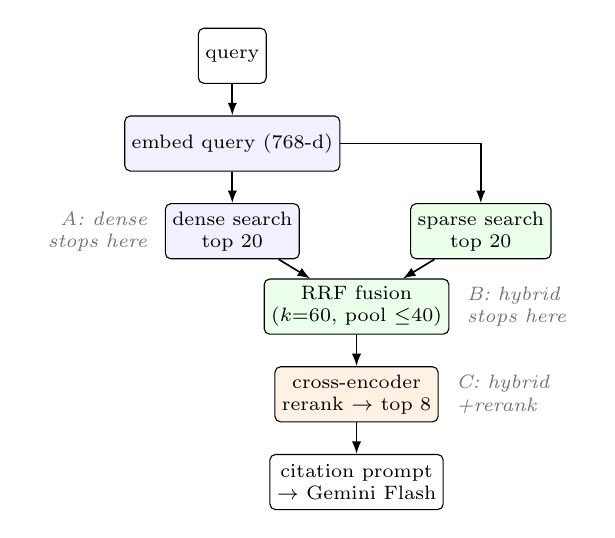
\begin{tikzpicture}[
  node distance=4mm and 6mm,
  box/.style={draw, rounded corners=2pt, align=center, font=\scriptsize,
              minimum height=7mm, inner sep=2.5pt},
  a/.style={fill=blue!6}, b/.style={fill=green!8}, c/.style={fill=orange!10},
  arr/.style={-{Latex[length=1.6mm]}, semithick},
  lbl/.style={font=\scriptsize\itshape, text=black!55}
]
\node[box] (q) {query};
\node[box, a, below=of q] (emb) {embed query (768-d)};
\node[box, a, below=of emb] (dense) {dense search\\top 20};
\node[box, b, right=14mm of dense] (sparse) {sparse search\\top 20};
\node[box, b, below=6mm of $(dense)!0.5!(sparse)$] (rrf) {RRF fusion\\($k{=}60$, pool $\le$40)};
\node[box, c, below=of rrf] (rer) {cross-encoder\\rerank $\rightarrow$ top 8};
\node[box, below=of rer] (gen) {citation prompt\\$\rightarrow$ Gemini Flash};

\draw[arr] (q) -- (emb);
\draw[arr] (emb) -- (dense);
\draw[arr] (emb.east) -| (sparse.north);
\draw[arr] (dense) -- (rrf);
\draw[arr] (sparse) -- (rrf);
\draw[arr] (rrf) -- (rer);
\draw[arr] (rer) -- (gen);

\node[lbl, left=1mm of dense, text width=14mm, align=right] {A: dense\\stops here};
\node[lbl, right=1mm of rrf, text width=14mm] {B: hybrid\\stops here};
\node[lbl, right=1mm of rer, text width=14mm] {C: hybrid\\+rerank};
\end{tikzpicture}
\caption{Retrieval pipeline. Method~A (dense) uses only the dense branch;
Method~B (hybrid) adds the sparse branch and RRF fusion (Eq.~\ref{eq:rrf});
Method~C adds cross-encoder reranking to the top~8
candidates under a per-source diversity cap. Generation is
identical for all three.}
\label{fig:pipeline}
\end{figure}

\section{Methodology}
\subsection{Corpus}
The test corpus consists of seven internal documents for a
fictitious company, "Infovance Technologies," spanning distinct enterprise
domains: an HR leave policy, an IT security policy, an IT helpdesk standard
operating procedure, a finance expense-reimbursement policy, an engineering team
handbook, an employee onboarding guide, and an IT incident report. The first six
are the sources for our questions; the seventh (the incident report) is included
in the searchable corpus but is not directly questioned, serving as an unqueried
distractor the retriever must rank against. The documents are clean,
well-structured policy text, representative of curated enterprise knowledge
bases. As we discuss later, this is an important determinant of our findings.

\subsection{Question set}
We authored 30 ground-truth question--answer pairs directly from the corpus, so
every question is answerable from the document text. Table~\ref{tab:questions}
gives the per-category breakdown. Twenty-six questions are answerable from a
single document ($\geq 4$ per source document); four are genuine
\emph{cross-document} questions whose answers require combining facts that each
live in only one document, stressing the retriever's ability to surface multiple
relevant sources at once.

\begin{table}[t]
\caption{Question set by category (30 total).}
\label{tab:questions}
\centering
\footnotesize
\begin{tabular}{@{}lc@{}}
\toprule
\textbf{Category (source document)} & \textbf{\# Questions} \\
\midrule
HR (Leave Policy)                          & 5 \\
IT Security (Security Policy)              & 4 \\
IT Helpdesk (Helpdesk SOP)                 & 4 \\
Finance (Expense Reimbursement Policy)     & 5 \\
Engineering (Team Handbook)                & 4 \\
Onboarding (Employee Onboarding Guide)     & 4 \\
Cross-document (two sources)               & 4 \\
\midrule
\textbf{Total}                             & \textbf{30} \\
\bottomrule
\end{tabular}
\end{table}

\subsection{Metrics}
We report two retrieval-sensitive RAG metrics, each in $[0,1]$:
\begin{itemize}
  \item \textbf{Faithfulness}: the fraction of the generated answer's claims that
        are supported by (entailed by) the retrieved context. It penalizes
        hallucinated claims not grounded in retrieved text.
  \item \textbf{Context precision}: the degree to which the retrieved context
        relevant to the question is concentrated, i.e.\ whether the retrieved
        passages are on-topic rather than padded with irrelevant material.
\end{itemize}
We summarize each method by the mean of the two metrics, following the project's
reporting convention.

\subsection{Independent-judge design}
A central methodological choice is that the model that \emph{generates} answers
is never the model that \emph{scores} them. Answers for all three conditions are
generated by Gemini Flash (\texttt{gemini-3.1-flash-lite}). Faithfulness is
scored by a locally hosted \texttt{qwen2.5:7b} model (via Ollama); context
precision is scored by \texttt{llama-3.1-8b-instant} (via Groq). Using two
distinct, independent judges, neither of which is the generator, removes the
self-evaluation bias in which a model systematically rates its own outputs
favourably.

\subsection{Evaluation asymmetries (disclosed)}
We disclose two asymmetries honestly, as both bear on interpretation.

\emph{Judge context depth (K-asymmetry).} The faithfulness judge scores against
the top 2 retrieved contexts and the context-precision judge against the top 3.
For all three methods this is a strict subset of the available contexts: Methods~A
and~B return around 7--8 contexts and Method~C returns about 4 (mean 4.17; see
Section~\ref{sec:results}). The two judges therefore see overlapping but not
identical material for every method. We return to whether this confounds the
reranking result in Section~\ref{sec:discussion}.

\emph{Coverage.} Every cell in Table~\ref{tab:results} is computed over the full
30 questions: all three methods answered all 30, and both judges scored all 30
for each method, with no timeouts or missing values.

\section{Results}
\label{sec:results}
Table~\ref{tab:results} reports faithfulness, context precision, and their
average for the three methods, with the exact values from the evaluation run.
Fig.~\ref{fig:bars} visualizes the two metrics across methods.

\begin{table}[t]
\caption{Retrieval-strategy comparison. Faithfulness scored by
\texttt{qwen2.5:7b} (top-2 contexts); context precision by
\texttt{llama-3.1-8b-instant} (top-3 contexts). Generator:
\texttt{gemini-3.1-flash-lite}. Best average in \textbf{bold}.}
\label{tab:results}
\centering
\footnotesize
\begin{tabular}{@{}lccc@{}}
\toprule
\textbf{Method} & \textbf{Faithfulness} & \textbf{Ctx.\ Precision} & \textbf{Avg.} \\
\midrule
A: Dense           & 0.873          & 0.933          & 0.903 \\
B: Hybrid          & \textbf{0.890} & \textbf{0.939} & \textbf{0.914} \\
C: Hybrid$+$Rerank & 0.777          & 0.903          & 0.840 \\
\bottomrule
\end{tabular}
\\[2pt]
\begin{minipage}{0.95\linewidth}
\footnotesize All cells are means over the full 30 questions; both judges scored
all 30 for every method.
\end{minipage}
\end{table}

Three observations follow directly from the data.

\textbf{(1) Hybrid attains the best average, but by a small margin.}
Hybrid's average (0.914) edges out dense (0.903) by 0.011, and crucially the two
per-metric values now point the \emph{same} way: hybrid is higher on both
faithfulness (0.890 vs.\ 0.873) and context precision (0.939 vs.\ 0.933). The
improvement is consistent in direction but modest in magnitude on $n=30$, and we
do not claim statistical significance; we read it as a small, real gain rather
than a decisive one.

\textbf{(2) The sparse channel is active and changes retrieval.} Inspecting the
retrieved contexts per question, dense (A) and hybrid (B) now return
\emph{different} context sets on all 30 of 30 questions: adding the sparse
retriever and RRF fusion reorders or substitutes at least one context everywhere.
This propagates to the metrics. The context-precision judge, given a fixed context
set, is deterministic, so its A-vs-B differences are pure retrieval effects: the
two methods earn different context-precision scores on 12 of 30 questions, and
hybrid's higher mean (0.939 vs.\ 0.933) is therefore a genuine retrieval
difference, not judging noise or a coverage artifact. Faithfulness, which is
answer-dependent, differs on 5 of 30 questions. This reverses the conclusion of
the earlier, defective draft, in which A and B retrieved byte-identical contexts
because the sparse channel was silently inert (Section~\ref{sec:methods}); under
the corrected implementation the lexical channel demonstrably contributes.

\textbf{(3) Reranking degrades both metrics.} Method~C's faithfulness
falls to 0.777 (0.096 below dense and 0.113 below hybrid), and its context
precision also drops to 0.903, giving the worst average (0.840) by a wide margin.
The cause is visible in the retrieved-context counts: Methods~A and~B return a
mean of about 7--8 contexts per question (A: 6.97, B: 7.60), whereas Method~C
returns a mean of 4.17 (range 4--5). Reranking to the top 8 under a per-source
diversity cap, followed by parent-text deduplication, roughly halves the context
available to the generator.

\begin{figure}[t]
\centering
\definecolor{faithblue}{RGB}{47,72,94}
\definecolor{ctxochre}{RGB}{198,166,118}
\begin{tikzpicture}
\begin{axis}[
  ybar,
  width=\linewidth,
  height=5cm,
  bar width=14pt,
  enlarge x limits=0.22,
  ymin=0.6, ymax=1.0,
  ytick={0.6,0.7,0.8,0.9,1.0},
  yticklabel style={font=\scriptsize, /pgf/number format/fixed,
                    /pgf/number format/precision=1},
  ylabel={Score},
  ylabel style={font=\footnotesize},
  ymajorgrids=true,
  grid style={draw=black!20, line width=0.4pt},
  symbolic x coords={Dense (A), Hybrid (B), Hybrid+Rerank (C)},
  xtick=data,
  x tick label style={font=\scriptsize},
  tick align=outside,
  tick style={black!55, line width=0.4pt},
  axis line style={black!55, line width=0.6pt},
  nodes near coords,
  nodes near coords style={font=\scriptsize, text=black!55, inner sep=1pt,
        /pgf/number format/fixed, /pgf/number format/precision=3},
  legend style={at={(0.5,-0.14)}, anchor=north, legend columns=-1,
                font=\scriptsize, draw=none, fill=none,
                /tikz/every even column/.append style={column sep=12pt}},
]
\addplot[fill=faithblue, draw=faithblue!80!black] coordinates {
  (Dense (A), 0.873) (Hybrid (B), 0.890) (Hybrid+Rerank (C), 0.777)};
\addplot[fill=ctxochre, draw=ctxochre!70!black] coordinates {
  (Dense (A), 0.933) (Hybrid (B), 0.939) (Hybrid+Rerank (C), 0.903)};
\legend{Faithfulness, Context precision}
\end{axis}
\end{tikzpicture}
\caption{Faithfulness and context precision by method. Hybrid is slightly above
dense on both metrics; reranking degrades both, with the largest drop in
faithfulness (0.873/0.890 $\rightarrow$ 0.777).}
\label{fig:bars}
\end{figure}

\section{Discussion}
\label{sec:discussion}
\subsection{Why reranking hurts here: context over-pruning}
The headline finding is that adding a cross-encoder reranker, conventionally
expected to improve precision, instead degraded faithfulness by 0.10 absolute.
The mechanism is over-pruning. The reranker keeps the top 8 candidates under a
per-source diversity cap, and the generation stage then deduplicates by parent
text. Because our hierarchical children overlap and many map to the same parent,
the reranked children collapse to fewer distinct parent blocks. Empirically, this
is a mean of 4.17 contexts for Method~C versus about 7--8 for Methods~A and~B,
roughly halving the material reaching the generator. With less surrounding
context to support every claim it makes, more of the answer goes ungrounded and
faithfulness falls.

This is a genuine property of the method on this corpus, not merely a measurement
artifact. The reduction to about four contexts is produced by the pipeline itself
(the reranker's top-8 cut and diversity cap composed with parent deduplication)
and would feed the same thinned context to the generator regardless of how it is
scored. On a small, clean corpus where the un-reranked pool is already highly
relevant, aggressive top-$k$ pruning removes useful redundant context without
removing meaningful noise, so the precision gain reranking is meant to provide has
little to bite on while the recall loss directly harms grounding.

\subsection{On the K-asymmetry}
We disclosed that the faithfulness judge sees the top 2 contexts and the
context-precision judge the top 3, while Method~C produces about 4 contexts in
total. This asymmetry could, in principle, inflate or deflate Method~C's scores
relative to A and~B, and we do not claim the absolute 0.777 is free of it.
However, the asymmetry does not manufacture the finding: the over-pruning that
drives the faithfulness drop is a real reduction in the context \emph{available
to the generator} (mean 4.17 blocks versus 7--8), which happens before any judge
is applied. A uniform-$K$ re-run would tighten the absolute numbers, but the
generator is grounded on the same thinned context either way.

\subsection{On the hybrid-vs-dense difference}
We report hybrid as the best method by average, consistent with its 0.914 mean,
and we are equally clear that the margin over dense (0.011) is small. What the
corrected run establishes is that the difference is \emph{real} rather than an
artifact: hybrid retrieves different contexts from dense on all 30 questions and
is nominally ahead on both metrics, and because the context-precision judge is
deterministic given a context set, hybrid's higher context precision (0.939 vs.\
0.933, differing on 12 of 30 questions) is attributable to retrieval, not to
scoring noise or coverage. We nonetheless refrain from significance claims at
$n=30$: the gain is consistent in direction but modest, and on this clean
policy corpus---where exact rare tokens are scarce---dense semantic matching
already retrieves most relevant passages, leaving the lexical channel limited
headroom. A corpus richer in abbreviations, identifiers, and codes, where lexical
matching is known to help, and a learned sparse encoder (SPLADE, FastEmbed BM25)
in place of our hashed term-frequency approximation would be needed to test
hybrid's advantage at full strength.

\subsection{Takeaway}
The practical lesson is that retrieval-stage value is contingent on corpus
characteristics. On a small, clean, semantically well-separated enterprise
corpus, dense retrieval alone is already strong; adding a sparse channel yields a
small but consistent improvement; and an aggressive reranker can actively hurt by
starving the generator of context. Reranking is not a free improvement to be
applied by default: its top-$k$ cut must be sized against the corpus and the
downstream context budget.

\section{Conclusion}
We used Pragya, a working enterprise RAG platform, as a controlled testbed to
compare dense, hybrid, and hybrid$+$rerank retrieval on a real seven-document
corporate corpus and 30 ground-truth questions, scored by two judge models
independent of the answer generator. Hybrid retrieval achieved the best average
score (0.914), ahead of dense (0.903) on both metrics on retrieved context that
differed from dense on every question, so the sparse channel's contribution is
small but real on this corpus. Cross-encoder reranking was clearly worst, dropping
faithfulness from 0.873 to 0.777 by over-pruning the generator's context to about
four blocks. These results caution against treating each additional retrieval
stage as a uniform improvement: on small, clean enterprise corpora, dense
retrieval is already strong and aggressive reranking can degrade faithfulness.
The value of hybrid retrieval and reranking is contingent on corpus
characteristics, and should be measured per deployment rather than assumed.

Three directions follow directly from the limitations disclosed above. A
uniform-$K$ evaluation, in which both judges score the same number of contexts,
would remove the disclosed K-asymmetry and report reranking's effect under
matched conditions, while replacing the sparse channel's hashed term-frequency
approximation with a learned encoder (SPLADE, or a FastEmbed BM25
implementation) would let the lexical channel's full contribution be measured
beyond our approximation. Finally, evaluation
on a larger, noisier corpus (with redundant and off-topic documents, where
lexical matching has rare tokens to catch and reranking has real noise to
remove) would test whether the negative reranking result is specific to small,
clean corpora.

\bibliographystyle{IEEEtran}
\bibliography{references}

\end{document}